\bookchapter{第四十二章：大模型全景同 API 實戰}

\chapterintro{前面幾章講嘅都係「點樣同 AI 協作」，本章解決一個更基礎嘅問題：「用邊個 AI？點樣用？」2026 年 8 月嘅大模型格局已經極其豐富——國際有 GPT、Claude、Gemini 三強爭霸，國內有 DeepSeek、通義千問、GLM、Kimi、豆包百花齊放。每個模型都有自己嘅性格同特長：揀啱咗事半功倍，揀錯咗事倍功半。本章唔單止帶你認識呢啲模型，仲會教你點樣透過 API 將佢哋接入自己嘅應用，以及點樣根據自己嘅需求揀合適嘅 Token Plan（用量套餐）。}

\booksection{一、國際主流大模型：三強格局}

2026 年 8 月嘅國際大模型市場，形成咗 OpenAI（GPT 系列）、Anthropic（Claude 系列）、Google（Gemini 系列）三強鼎立嘅格局。每家都有自己鮮明嘅特色——我哋一個一個認識。

\booksubsection{OpenAI GPT-5.6 系列：全能均衡嘅六邊形戰士}

OpenAI 係大模型浪潮嘅開啟者，GPT 系列至今仍然係全球使用最廣泛嘅模型。2026 年 7 月發佈嘅 GPT-5.6 系列採用三檔定位策略：旗艦款 GPT-5.6 Sol 面向高端推理需求，均衡款 GPT-5.6 Terra 面向日常開發，輕量款 GPT-5.6 Luna 面向高並發低成本場景。三款模型共享 105 萬 Token 嘅上下文視窗，都支援圖像輸入、函數調用同結構化輸出。

\begin{center}
\begin{tabularx}{\linewidth}{|X|X|X|X|X|}
\hline
\textbf{型號} & \textbf{定位} & \textbf{輸入(/百萬Token)} & \textbf{輸出(/百萬Token)} & \textbf{上下文視窗} \tabularnewline
\hline
GPT-5.6 Sol & 旗艦推理 & US\$5.00（約36蚊） & US\$30.00（約217蚊） & 105萬Token \tabularnewline
GPT-5.6 Terra & 均衡日常 & US\$2.50（約18蚊） & US\$15.00（約109蚊） & 105萬Token \tabularnewline
GPT-5.6 Luna & 輕量低成本 & US\$1.00（約7蚊） & US\$6.00（約44蚊） & 105萬Token \tabularnewline
\hline
\end{tabularx}
\end{center}

\begin{center}\small\color{gray}OpenAI GPT-5.6 系列定價（2026 年 8 月）\end{center}

GPT 系列嘅核心優勢喺於「均衡」——推理、編程、寫作、多模態，冇明顯短板。加上 OpenAI 龐大嘅插件生態同開發者社區，適配文檔同工具鏈最為完善。對於「唔知揀乜嘢」嘅場景，GPT 係「盲揀都唔會錯」嘅預設答案。但佢嘅短板係：國內訪問需要特殊網絡，中文表達偶爾有「翻譯腔」，API 價格處於中高水平。

\textbf{好消息}\par

OpenAI 喺 2026 年 8 月宣佈免費用戶預設模型升級為 GPT-5.6 Luna，並開放無限量文本聊天。呢個意味住你可以零成本體驗 GPT 嘅基礎能力，只有喺需要更強推理或者 API 調用時先需要付費。

\booksubsection{Anthropic Claude 系列：編程同嚴謹嘅天花板}

如果話 GPT 係全能選手，咁 Claude 就係編程領域嘅「天花板」。Anthropic 嘅 Claude 系列喺 SWE-bench（軟件工程基準測試）上長期斷層領先，代碼生成質量同工程級項目落地能力業界第一。更難得嘅係，Claude 嘅幻覺率（生成虛假資訊嘅概率）全網最低，僅約 1\%——呢個令佢特別適合學術、法務等高精度場景。

Claude 嘅另一個殺手鐧係超長上下文：支援 100 萬 Token 嘅上下文視窗，能夠一次性「讀完」幾百頁嘅合約或者成個代碼庫唔漏細節。呢個喺代碼重構、長文檔分析等場景中幾乎無可替代。Claude Code 作為終端 AI 編程工具，到 2026 年中期年化收入已達 25 億美元——呢個係 Claude 編程能力最受認可嘅證據。

\begin{center}
\begin{tabularx}{\linewidth}{|X|X|X|X|X|}
\hline
\textbf{型號} & \textbf{定位} & \textbf{輸入(/百萬Token)} & \textbf{輸出(/百萬Token)} & \textbf{上下文視窗} \tabularnewline
\hline
Claude Fable 5 & 旗艦款 & US\$10.00（約72蚊） & US\$50.00（約362蚊） & 100萬Token \tabularnewline
Claude Opus 4.8 & 專業款 & US\$5.00（約36蚊） & US\$25.00（約181蚊） & 100萬Token \tabularnewline
Claude Sonnet 5 & 性價比款 & US\$2.00（約14蚊） & US\$10.00（約72蚊） & 100萬Token \tabularnewline
\hline
\end{tabularx}
\end{center}

\begin{center}\small\color{gray}Anthropic Claude 系列定價（2026 年 8 月，Sonnet 5 為優惠價）\end{center}

Claude 嘅短板係價格——Fable 5 嘅輸出價格係所有模型中最高嘅，每百萬 Token 要 50 美元。多模態能力（圖像、視像理解）亦相對較弱。對於預算有限嘅個人開發者，Sonnet 5 喺優惠期內嘅性價比非常突出。

\booksubsection{Google Gemini 系列：多模態嘅王者}

Google 嘅 Gemini 系列喺 2026 年已迭代至 3.1 Pro 版本。Gemini 嘅最大殺手鐧係原生多模態——圖文解析精準、OCR 表格識別無誤、視像幀提取高效，仲支援音視像深度解析。佢同 Google 生態（搜尋、電郵、雲服務）深度綁定，喺即時資訊檢索同跨模態理解上表現突出。Gemini 仲支援 200 萬 Token 嘅超長上下文輸入，係目前上下文視窗最大嘅模型。

Gemini 嘅定位係「科學推理同多模態場景嘅首選」。如果你嘅項目涉及大量圖像分析、視像理解或者科學計算，Gemini 幾乎冇對手。但佢喺純文本代碼生成上略遜於 Claude，中文表達亦不如國產模型自然。

\begin{center}
\begin{tabularx}{\linewidth}{|X|X|X|X|}
\hline
\textbf{對比項目} & \textbf{GPT-5.6} & \textbf{Claude Fable 5} & \textbf{Gemini 3.1 Pro} \tabularnewline
\hline
綜合得分 & 94.8 & 95.0 & 92.1 \tabularnewline
編程能力(SWE-bench) & 74.9\% & 64.3\% (Pro) & 中等 \tabularnewline
上下文視窗 & 105萬Token & 100萬Token & 200萬Token \tabularnewline
多模態能力 & 均衡 & 較弱 & 最強 \tabularnewline
幻覺率 & 較低 & 最低(約1\%) & 較低 \tabularnewline
國內可用性 & 需特殊網絡 & 需特殊網絡 & 需特殊網絡 \tabularnewline
API 生態 & 最完善 & 成長中 & Google 生態綁定 \tabularnewline
\hline
\end{tabularx}
\end{center}

\begin{center}\small\color{gray}國際三大模型橫向對比（2026 年 8 月）\end{center}

\begin{tcbwarn}{留意：國內使用嘅現實門檻}
對於國內開發者來說，GPT、Claude、Gemini 嘅核心障礙係網絡訪問。雖然可以透過 Azure 代理、API 聚合平臺等方式間接使用，但穩定性同合規性需要自行評估。如果你嘅項目對數據安全有嚴格要求，建議優先考慮國產模型。

\end{tcbwarn}

\booksection{二、國產主流大模型：百花齊放}

2026 年嘅國產大模型已經由「追趕者」變成「並跑者」，喺某些領域甚至實現咗「領跑」。同 2023 年「套殼」爭議唔同，2026 年嘅國產旗艦模型喺邏輯推理、代碼生成、中文理解等方面已經同國際一線模型旗鼓相當，差距縮減到 5\% 以內。更重要嘅係，國產模型喺中文場景、價格成本同合規部署上有不可替代嘅優勢。

\booksubsection{DeepSeek V4：性價比之王}

DeepSeek（深度求索）係國產大模型中現象級嘅存在。2025 年初，DeepSeek-V3 以「比 GPT 平十分之一但能力相當」嘅定位震撼市場，被業內稱為「通用 AI 大模型斬殺線」——比佢平嘅冇佢好用，比佢貴嘅冇佢量大管飽。到 2026 年 8 月，DeepSeek V4-Pro 正式版發佈：1.6 萬億參數 MoE 架構，激活約 49B，支援 100 萬無損上下文，代碼性價比被廣泛認為係全球天花板。

DeepSeek V4 喺 Agent 能力上實現咗大幅躍升——DeepSWE 基準由 12.8 跳至 62.7（+390\%），NL2Repo 由 38.5 升至 61.5。API 新增咗 Responses API 同 Anthropic API 雙協議支援，已兼容 Codex 同 Claude Code 等主流編程工具。呢個意味住你可以用 DeepSeek 嘅 API 替代 Claude 嘅 API，喺 Claude Code 中使用——成本降低數倍，體驗幾乎一致。

\begin{center}
\begin{tabularx}{\linewidth}{|X|X|X|X|X|}
\hline
\textbf{型號} & \textbf{定位} & \textbf{輸入(/百萬Token)} & \textbf{輸出(/百萬Token)} & \textbf{上下文視窗} \tabularnewline
\hline
DeepSeek V4 Pro & 旗艦推理 & 3蚊（約US\$0.43） & 6蚊（約US\$0.87） & 100萬Token \tabularnewline
DeepSeek V4 Flash & 輕量快速 & 1蚊（約US\$0.14） & 2蚊（約US\$0.28） & 100萬Token \tabularnewline
\hline
\end{tabularx}
\end{center}

\begin{center}\small\color{gray}DeepSeek V4 系列定價（2026 年 8 月，促銷價）\end{center}

價格對比：同樣 100 萬 Token 嘅輸入 + 100 萬 Token 嘅輸出，DeepSeek V4 Flash 花費約 0.42 美元，GPT-5.6 Sol 花費約 35 美元，Claude Fable 5 花費約 60 美元。差距高達 80-140 倍。

\textbf{避坑提醒：DeepSeek 要加價喇}\par

DeepSeek 官方已於 2026 年 8 月 6 日公告「計劃近期大幅上調 API 定價」，促銷價可能唔會持續太久。部分媒體傳聞漲幅可能達 30 倍，截至 8 月 14 日官方尚未公佈最終調價方案。此外，DeepSeek V4 正式版引入咗峯谷定價機制——高峯時段調用價格直接翻倍。建議關注官方公告獲取最新定價。

\booksubsection{通義千問 Qwen3.7 Max：阿里雲嘅企業級選擇}

阿里雲嘅通義千問（Qwen）系列依託阿里雲生態，喺企業級部署上有天然優勢。2026 年 7 月嘅 Qwen3.7 Max 係當前旗艦：235B 參數稠密模型，256K 原生上下文，可擴展至 1M。Qwen 嘅核心優勢喺於：開源生態成熟（由 7B 到 235B 全系列開源）、中文場景理解精準、同阿里雲基礎設施深度整合。

\begin{center}
\begin{tabularx}{\linewidth}{|X|X|X|}
\hline
\textbf{型號} & \textbf{輸出價格(/百萬Token)} & \textbf{適用場景} \tabularnewline
\hline
qwen-turbo & 0.6蚊 & 極簡問答、文本分類、高並發 \tabularnewline
qwen-long & 2.0蚊 & 10M 超長上下文處理 \tabularnewline
qwen3.7-flash & 7.2蚊 & 通用對話、內容生成 \tabularnewline
qwen3.7-plus & 12.0蚊 & 多模態（圖片+視像）、中文創作 \tabularnewline
qwen3.7-max & 36.0蚊 & 旗艦中文能力、複雜任務 \tabularnewline
\hline
\end{tabularx}
\end{center}

\begin{center}\small\color{gray}通義千問 Qwen 系列階梯定價（2026 年 8 月）\end{center}

Qwen 嘅定價採用階梯策略——由極低成本嘅 qwen-turbo（輸出 0.6 蚊/百萬 Token）到旗艦 qwen3.7-max（輸出 36 蚊/百萬 Token），覆蓋由輕量問答到複雜推理嘅全場景需求。對於已經喺度用阿里雲嘅企業，Qwen 係最順手嘅整合選擇。

\booksubsection{智譜 GLM-5.1：國產 SWE-bench 第一}

智譜 AI 嘅 GLM 系列喺 2026 年表現亮眼。GLM-5.1 喺 SWE-bench 上攞到國產第一嘅成績：744B MoE 稠密混合架構，支援 100 萬上下文。佢嘅特點係中文語義理解精準，支援國內合規私有化部署——呢個對數據安全要求高嘅金融、政務場景非常重要。GLM-5.1 嘅定價為輸入 6 蚊、輸出 24 蚊每百萬 Token，處於國產模型中游水平。

\booksubsection{Kimi K3：超長文本之王}

月之暗面嘅 Kimi 系列以超長文本處理能力著稱。2026 年 7 月發佈嘅 Kimi K3 擁有 2.8 萬億參數規模，喺多項複雜任務評測中進入全球第一梯隊。Kimi 嘅核心場景係長代碼庫分析同長文檔檢索增強——佢能夠處理成本書嘅文本或者成個項目嘅代碼，喺「大海撈針」式檢索任務中表現卓越。Kimi 嘅定價相對較高（輸出約 12-20 蚊/百萬 Token），但喺長文本場景嘅性價比無人能及。

\booksubsection{豆包 Doubao：字節跳動嘅全能選手}

字節跳動嘅豆包系列喺 2026 年表現穩定。Doubao Seed 2.1 Pro 係火山引擎旗艦模型，256K 上下文，喺實測中綜合發揮穩定，中文場景體驗突出。豆包嘅優勢喺於：註冊即送大量免費 Token，火山引擎生態整合完善，定價處於國內最低梯隊之一。對於想要快速體驗 AI 編程嘅初學者，豆包係零門檻嘅入門選擇。

\begin{center}
\begin{tabularx}{\linewidth}{|X|X|X|X|X|X|}
\hline
\textbf{對比項目} & \textbf{DeepSeek V4} & \textbf{Qwen3.7 Max} & \textbf{GLM-5.1} & \textbf{Kimi K3} & \textbf{豆包 2.1 Pro} \tabularnewline
\hline
綜合得分 & 87.5 & 89.7 & 90.5 & 88+ & 85+ \tabularnewline
編程能力 & 極強 & 強 & 國產SWE第一 & 強 & 中上 \tabularnewline
中文理解 & 優秀 & 優秀 & 精準 & 優秀 & 優秀 \tabularnewline
上下文視窗 & 100萬 & 256K-1M & 100萬 & 超長 & 256K \tabularnewline
輸出價格(蚊/M) & 6 & 36 & 24 & 12-20 & 30 \tabularnewline
開源 & MIT協議 & 全系列開源 & 部分開源 & 閉源 & 閉源 \tabularnewline
私有化部署 & 支援 & 支援 & 支援 & 唔支援 & 唔支援 \tabularnewline
\hline
\end{tabularx}
\end{center}

\begin{center}\small\color{gray}國產五大模型橫向對比（2026 年 8 月）\end{center}

一個重要嘅趨勢係：國產模型同 GPT/Claude 嘅「代差感」已經消失。喺邏輯推理同數學競賽上，國產旗艦同 GPT-5 嘅分差基本上喺個位數。喺系統化架構思維同複雜工程推理上，Claude 仍然領先——佢能夠畀出更有「靈氣」嘅架構方案，而國產模型有時顯得「教條」。但喺中文場景、成本控制同合規部署上，國產模型有壓倒性優勢。

\begin{center}
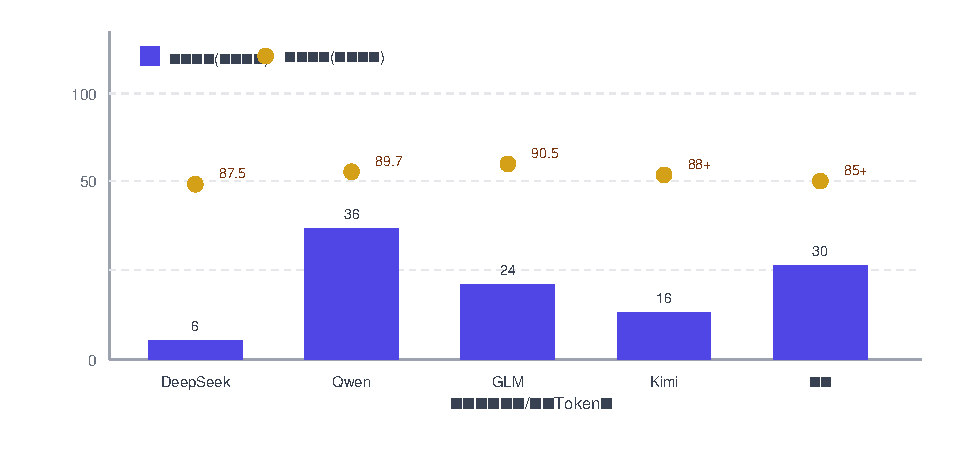
\includegraphics[width=0.92\linewidth]{figures/fig-di-si-shi-er-zhang-1}
\\[2pt]\small 圖 4：五款模型嘅價格同性能對比（價格越低越好，得分越高越好）
\end{center}

\booksection{三、模型選擇決策框架}

瞭解咗各模型嘅特點之後，點樣為自己嘅項目揀模型？呢度送你一套「四問決策法」——回答四個問題，就能夠鎖定最適合你嘅模型。

你個項目係喺國內定係國際部署？

國內 選國產模型

|

國際 可選海外模型

核心任務係編程定係其他？

編程 Claude 或 DeepSeek

|

其他 繼續判斷

需要超長上下文(>50萬Token)？

需要 Gemini 或 Kimi

|

不需要 繼續判斷

使唔使考慮預算？

敏感 DeepSeek 或 Qwen-turbo

|

不敏感 GPT-5.6 或 Claude

\begin{center}\small\color{gray}圖 5：大模型選擇四問決策法\end{center}

\begin{tcbinfo}{小貼士：組合策略}
呢個決策法唔係教條——好多場景需要組合使用多個模型。一個常見嘅組合策略：用 DeepSeek 或者 Qwen 做日常開發（成本低、中文好），用 Claude 做關鍵架構設計（推理強、幻覺低），用 Gemini 做多模態分析（圖像視像處理）。按需切換模型，而唔係「一個模型用到死」。

\end{tcbinfo}

\booksection{四、API 調用入門：由零開始接入大模型}

好多 AI 編程教程只教你點樣用對話介面，但真正嘅「AI 編程」——令你嘅應用調用大模型——需要透過 API。API（Application Programming Interface，應用程序編程接口）係程序之間嘅通訊協議。透過 API，你嘅代碼可以好似調用一個函數一樣，調用大模型嘅能力。

\booksubsection{Token 係乜嘢}

喺瞭解 API 之前，必須先理解「Token」呢個概念。Token 係大模型計費嘅基本單位，可以理解為「AI 嘅閱讀同寫作單位」。一個 Token 大約對應：英文中 0.75 個單詞（4 個字符），中文中 0.5-1 個漢字。一段 1000 字嘅中文文本，大約消耗 1500-2000 個 Token。

Token 唔係字數，亦唔係字符數。大模型使用專門嘅分詞器（Tokenizer）將文本切分成 Token。同一個詞喺唔同模型中嘅 Token 數量可能唔同——例如「人工智能」喺 GPT 中可能係 3 個 Token，喺 DeepSeek 中可能係 2 個。大多數模型嘅 API 會返回實際消耗嘅 Token 數量，你可以喺 API 響應中查看。

\begin{tcbinfo}{Token 成本快速估算}
100 萬字中文約等於 150 萬 Token。用 DeepSeek V4 Flash 處理 100 萬字輸入 + 100 萬字輸出，成本約 0.42 美元（約 3 蚊人民幣）；用 Claude Fable 5 處理同樣嘅量，成本約 60 美元（約 434 蚊人民幣）。呢個就係點解模型選擇直接影響你嘅項目成本。

\end{tcbinfo}

\booksubsection{取得 API Key}

使用大模型 API 嘅第一步係取得 API Key——一串用嚟做身份驗證嘅密鑰。每個模型供應商都有自己嘅 API 平臺，你需要註冊帳號並創建 API Key。以下係主流模型嘅 API 平臺入口同獲取流程：

\begin{center}
\begin{tabularx}{\linewidth}{|X|X|X|X|}
\hline
\textbf{模型} & \textbf{API 平臺} & \textbf{獲取流程} & \textbf{免費額度} \tabularnewline
\hline
DeepSeek & platform.deepseek.com & 註冊 實名認證 創建 API Key & 新用戶贈送額度 \tabularnewline
通義千問 & bailian.aliyun.com（百煉平臺） & 阿里雲帳號登入 開通服務 創建 Key & 新用戶免費試用 \tabularnewline
智譜GLM & open.bigmodel.cn & 註冊 實名認證 創建 API Key & 新用戶贈送額度 \tabularnewline
Kimi & platform.moonshot.cn & 註冊 實名認證 創建 API Key & 有限免費額度 \tabularnewline
豆包 & volcengine.com（火山引擎） & 註冊 開通方舟 創建 API Key & 註冊送大量 Token \tabularnewline
OpenAI GPT & platform.openai.com & 註冊 綁定信用卡 創建 API Key & 冇免費額度（要付費） \tabularnewline
Anthropic Claude & console.anthropic.com & 註冊 綁卡 創建 API Key & 新用戶少量額度 \tabularnewline
\hline
\end{tabularx}
\end{center}

\begin{center}\small\color{gray}主流模型 API 平臺同 Key 獲取方式（2026 年 8 月）\end{center}

\textbf{安全提示：API Key = 銀包密碼}\par

API Key 等同於你嘅銀包密碼——任何拎到 Key 嘅人都可以用你嘅額度調用模型。因此：永遠唔好將 API Key 寫喺代碼中（用環境變數管理）；永遠唔好將含 Key 嘅代碼提交到公開嘅 Git 倉庫；永遠唔好喺社交媒體分享含 Key 嘅截圖。如果 Key 洩露咗，即刻喺平臺上刪除並重新創建。

\booksubsection{第一次 API 調用}

取得 API Key 之後，你可以用任何編程語言調用大模型 API。以下用 Python 演示一個最簡單嘅調用——向 DeepSeek 發送一條訊息並攞回覆。

\begin{lstlisting}[language=Python]
# 安裝SDK：pip install openai
# DeepSeek兼容OpenAI SDK格式，可以直接用
from openai import OpenAI
import os

# 1. 建立客戶端（API Key從環境變數讀取）
client = OpenAI(
    api_key=os.environ.get("DEEPSEEK_API_KEY"),
    base_url="https://api.deepseek.com"
)

# 2. 發送請求
response = client.chat.completions.create(
    model="deepseek-chat",  # 指定模型
    messages=[
        {"role": "system", "content": "你係一個Python編程助手。"},
        {"role": "user", "content": "寫一個快速排序函數。"}
    ]
)

# 3. 攞回覆
print(response.choices[0].message.content)

# 4. 睇Token消耗
print(f"輸入Token: {response.usage.prompt_tokens}")
print(f"輸出Token: {response.usage.completion_tokens}")
print(f"總Token: {response.usage.total_tokens}")
\end{lstlisting}

呢段代碼嘅核心邏輯係：創建用戶端（帶住 API Key 同模型地址） 構造訊息列表（system 設定角色，user 係用戶輸入） 發送請求 攞回覆。呢個模式幾乎適用於所有兼容 OpenAI 格式嘅模型——只需要更換 api\_key 同 base\_url 就能夠切換模型。呢個就係點解好多國產模型揀兼容 OpenAI SDK 格式：開發者只需改兩行代碼就能夠切換模型，遷移成本極低。

以下係切換到其他模型嘅代碼差異——留意只需要改兩行：

\begin{lstlisting}[language=Python]
# DeepSeek
client = OpenAI(
    api_key=os.environ.get("DEEPSEEK_API_KEY"),
    base_url="https://api.deepseek.com"
)
# model="deepseek-chat"

# 通義千問（百鍊平臺）
client = OpenAI(
    api_key=os.environ.get("DASHSCOPE_API_KEY"),
    base_url="https://dashscope.aliyuncs.com/compatible-mode/v1"
)
# model="qwen-plus"

# 智譜GLM
client = OpenAI(
    api_key=os.environ.get("GLM_API_KEY"),
    base_url="https://open.bigmodel.cn/api/paas/v4"
)
# model="glm-4"

# OpenAI GPT
client = OpenAI(
    api_key=os.environ.get("OPENAI_API_KEY"),
    # base_url使用預設值即可
)
# model="gpt-5.6-terra"
\end{lstlisting}

\booksubsection{流式響應處理}

喺實際應用中，你通常唔希望等 AI 寫完所有內容先至一次性顯示——咁樣會令用戶等太耐。流式響應（Streaming）可以令你喺 AI 生成嘅同時逐字顯示，大幅提升用戶體驗。就好似打字機一樣，字一個一個彈出嚟，用戶嘅感覺係完全唔同嘅。

\begin{lstlisting}[language=Python]
# 串流回應：逐字輸出
stream = client.chat.completions.create(
    model="deepseek-chat",
    messages=[
        {"role": "user", "content": "寫一個Python嘅冒泡排序教程"}
    ],
    stream=True  # 開啓流式響應
)

# 逐塊接收並打印
for chunk in stream:
    if chunk.choices[0].delta.content is not None:
        print(chunk.choices[0].delta.content, end="", flush=True)
# 輸出會好似打字機噉逐字顯示
\end{lstlisting}

\booksection{五、Token Plan 購買指南}

大多數模型供應商有兩種計費方式：按量計費（Pay-as-you-go）同套餐訂閱（Token Plan / Subscription）。理解呢兩種方式嘅區別，能夠幫你大幅降低使用成本。

\booksubsection{按量計費 vs 套餐訂閱}

\begin{center}
\begin{tabularx}{\linewidth}{|X|X|X|}
\hline
\textbf{維度} & \textbf{按量計費(Pay-as-you-go)} & \textbf{套餐訂閱(Subscription)} \tabularnewline
\hline
計費方式 & 用幾多 Token 付幾多錢 & 預付固定費用，獲得額度 \tabularnewline
適合場景 & 使用量唔穩定、偶爾調用 & 使用量穩定、高頻調用 \tabularnewline
價格優勢 & 標準價 & 平過按量計20\%-50\% \tabularnewline
靈活性 & 隨時可用，唔使承諾 & 需要預付，額度過期可能作廢 \tabularnewline
超額處理 & 自動按量計費 & 超出額度後轉為按量計費 \tabularnewline
代表平臺 & 各個模型嘅官方API平臺 & OpenAI Plus/Pro, Claude Pro, Cursor Pro \tabularnewline
\hline
\end{tabularx}
\end{center}

\begin{center}\small\color{gray}兩種計費方式嘅對比\end{center}

對於初學者，建議由按量計費開始——唔需要預付費用，用幾多花幾多。當你嘅月使用量穩定喺一個水平之後（例如每月超過 50 蚊），再考慮切換到套餐訂閱以獲得更低單價。

\booksubsection{主流訂閱套餐一覽}

\begin{center}
\begin{tabularx}{\linewidth}{|X|X|X|X|}
\hline
\textbf{套餐} & \textbf{月費} & \textbf{包含內容} & \textbf{適合人羣} \tabularnewline
\hline
ChatGPT Free & 免費 & GPT-5.6 Luna 無限文本對話 & 零基礎體驗 \tabularnewline
ChatGPT Plus & US\$20/月 & GPT-5.6 Sol、圖像生成、數據分析、插件訪問 & 中度用戶 \tabularnewline
ChatGPT Pro & US\$200/月 & 無限制使用所有模型、優先訪問新功能 & 重度專業用戶 \tabularnewline
Claude Free & 免費 & 有限次數Claude對話 & 零基礎體驗 \tabularnewline
Claude Pro & US\$20/月 & 無限制Claude使用、優先訪問新模型 & 編程開發者 \tabularnewline
Cursor Free & 免費 & 有限次數AI補全同對話 & 初學者體驗 \tabularnewline
Cursor Pro & US\$20/月 & 無限AI補全、500次/月進階請求 & 日常開發者 \tabularnewline
Cursor Business & US\$40/月/人 & 團隊協作、管理後臺、私隱模式 & 團隊使用 \tabularnewline
\hline
\end{tabularx}
\end{center}

\begin{center}\small\color{gray}主流 AI 工具訂閱套餐（2026 年 8 月）\end{center}

國內模型嘅訂閱方案略有唔同。DeepSeek 主要按量計費，冇月度訂閱套餐——你充值後按實際使用量扣費。通義千問喺百煉平臺提供預付費資源包（購買一定量嘅 Token 額度，享受折扣價）。豆包喺火山引擎上亦有類似嘅預付費方案。對於國內開發者，最經濟嘅組合通常係：DeepSeek 按量計費（日常開發）+ 豆包免費額度（體驗測試）。

\booksubsection{API 聚合平臺}

如果你需要同時使用多個模型，API 聚合平臺係一個慳心嘅選擇。聚合平臺提供一個統一嘅 API Key，你就能夠調用全球幾十種模型，唔使喺每個平臺分別註冊。

\begin{center}
\begin{tabularx}{\linewidth}{|X|X|X|X|}
\hline
\textbf{平臺} & \textbf{特點} & \textbf{價格優勢} & \textbf{適合場景} \tabularnewline
\hline
OpenRouter (openrouter.ai) & 海外聚合平臺，一個Key調用全球模型 & 價格透明，支援即時比價 & 需要靈活切換多個海外模型 \tabularnewline
SiliconFlow (siliconflow.cn) & 國內聚合平臺，提供多種國產模型API & 平過官方20\%-30\% & 國內開發者，多模型比價 \tabularnewline
Azure OpenAI（微軟代理） & 微軟Azure代理嘅OpenAI API & Batch API 可以打五折 & 企業級OpenAI調用，大批量非同步任務 \tabularnewline
百度千帆（qianfan.baidubce.com） & 百度AI雲平臺，提供文心等模型 & 新用戶送額度 & 百度生態用戶 \tabularnewline
\hline
\end{tabularx}
\end{center}

\begin{center}\small\color{gray}主流 API 聚合平臺（2026 年 8 月）\end{center}

\textbf{避坑提醒：唔好買「共享 Key」}\par

唔好喺淘寶、閒魚等平臺買啲所謂嘅「共享 API Key」——呢啲 Key 通常來路不明，隨時可能被封號，仲有資料外洩嘅風險。記住一定要經官方平臺或者正規聚合平臺攞 API Key。

\booksubsection{成本優化策略}

揀啱模型只係第一步，點樣「用得慳錢」同樣重要。以下係幾個經過實踐驗證嘅成本優化策略：

\begin{enumerate}
  \item 善用快取命中。好多模型都有「快取」功能——當你嘅請求包含之前處理過嘅內容（例如系統提示詞），呢部分只會用超低價錢計費。DeepSeek 嘅快取命中價錢只係普通價錢嘅 1/60。將固定嘅系統提示放喺訊息列表開頭，就可以令快取命中最大化。
  \item 分級路由——用平價模型處理簡單任務，貴價模型處理複雜任務。例如用 DeepSeek V4 Flash 做文本分類（輸出 2 元/百萬 Token），用 Claude 做架構設計（輸出 181 元/百萬 Token）。一個項目入面 80\% 嘅呼叫都可以用平價模型搞掂。
  \item 限制輸出長度。API 係按輸出 Token 計費，輸出越長越貴。喺唔需要長篇大論嘅場景，設定 max\_tokens 參數去限制輸出長度，免得 AI「廢話太多」。
  \item 用 Batch API 處理非實時任務。如果你有大量唔需要即時回應嘅任務（例如批量數據標註、檔案摘要），用 Batch API 可以平一半。OpenAI 同 Azure 都有呢個功能。
  \item 監察 Token 用量。大部分 API 平臺都有用量統計面板。定期睇嚇用量分佈，搵出消耗 Token 最多嘅呼叫，再針對性咁優化。小小一個 Prompt 調整（例如將「請詳細解釋」改成「請用 3 句話解釋」）隨時可以慳返 50\% 嘅 Token。
\end{enumerate}

\begin{center}
\begin{tabularx}{\linewidth}{|X|X|X|X|}
\hline
\textbf{優化策略} & \textbf{慳到幾多} & \textbf{實施難度} & \textbf{說明} \tabularnewline
\hline
快取命中 & 最高98\% & 低 & 將固定內容放喺訊息開頭 \tabularnewline
分級路由 & 50\%-80\% & 中 & 簡單任務用平價模型 \tabularnewline
限制輸出長度 & 30\%-60\% & 低 & 設定max\_tokens參數 \tabularnewline
Batch API & 50\% & 低 & 非實時任務用批處理 \tabularnewline
Prompt優化 & 20\%-50\% & 中 & 精簡Prompt，減少冗餘 \tabularnewline
\hline
\end{tabularx}
\end{center}

\begin{center}\small\color{gray}成本優化策略及效果（2026 年 8 月）\end{center}

\booksection{六、實戰：喺項目入面接入大模型 API}

等我哋用一個完整嘅實戰嚟完結呢一章——整一個「AI 摘要產生器」：用戶輸入一段長文本，呼叫大模型 API 產生摘要。呢個實戰會展示 API 呼叫嘅完整流程：環境配置、API 呼叫、錯誤處理、成本控制。

\begin{lstlisting}[language=Python]
# ai_summarizer.py - AI摘要生成器
import os
from openai import OpenAI

# 1. 配置（API Key從環境變數讀取，絕不硬編碼）
client = OpenAI(
    api_key=os.environ.get("DEEPSEEK_API_KEY"),
    base_url="https://api.deepseek.com"
)

def summarize(text: str, max_length: int = 200) -> dict:
    """生成文本摘要

    Args:
        text: 要摘要嘅原文
        max_length: 摘要最大長度（Token數）

    Returns:
        dict: 包含摘要同Token消耗資訊
    """
    try:
        response = client.chat.completions.create(
            model="deepseek-chat",
            messages=[
                {
                    "role": "system",
                    "content": "你係一個摘要生成器。"
                               "請用簡潔嘅中文總結用戶提供嘅文本。"
                               "摘要不超過3句話。"
                },
                {
                    "role": "user",
                    "content": f"請摘要以下文本:\n\n{text}"
                }
            ],
            max_tokens=max_length,  # 限制輸出長度
            temperature=0.3  # 低溫度=更穩定
        )

        return {
            "success": True,
            "summary": response.choices[0].message.content,
            "input_tokens": response.usage.prompt_tokens,
            "output_tokens": response.usage.completion_tokens,
            "total_tokens": response.usage.total_tokens
        }

    except Exception as e:
        return {
            "success": False,
            "error": str(e)
        }

# 2. 使用示例
if __name__ == "__main__":
    long_text = """
    （粘貼一段長文本...）
    """

    result = summarize(long_text)

    if result["success"]:
        print(f"摘要: {result['summary']}")
        print(f"消耗Token: {result['total_tokens']}")
        # 估算成本：DeepSeek V4 Flash
        cost = result['total_tokens'] * 0.000004  # 約0.4分/千Token
        print(f"預估成本: {cost:.4f}元")
    else:
        print(f"出錯咗: {result['error']}")
\end{lstlisting}

呢段代碼體現咗 API 呼叫嘅幾個最佳實踐：API Key 係透過環境變數讀取，絕對唔會寫死喺代碼入面；函數有清晰嘅文檔同類型提示；設定咗 max\_tokens 去限制輸出長度；temperature 設做低值（0.3）等輸出更穩定；有完整嘅錯誤處理；仲會傳回 Token 消耗資訊用嚟追蹤成本。當你用 AI 嚟寫呢段代碼嗰陣，可以話畀佢知呢啲要求——佢完全有能力幫你實現。

本章嘅最終啟示：模型係"彈藥"，方法論係"戰術"。揀啱彈藥可以令戰鬥順啲，但冇好戰術，幾勁嘅彈藥都打唔贏仗。瞭解到各模型嘅特點同 API 用法之後，你就有一個充足嘅"彈藥庫"——但係點樣打呢場仗，仲係要靠前幾章學到嘅思維方法論。

\begin{tcbpractice}{嚟動手：搞掂你嘅第一次 API 呼叫}
註冊一個國產模型平臺（推薦 DeepSeek 或者智譜，兩家都送新用戶額度），整一個 API Key，將佢寫入系統環境變數（唔好寫入代碼入面！），然後行嚇上面「第一次 API 呼叫」嘅代碼。睇到 AI 嘅回覆打印出嚟嗰一刻，你就跨過咗「用 AI」同「整 AI 應用」之間嘅分界線。

\end{tcbpractice}

\begin{tcbsummary}{本章小結}
\begin{itemize}
  \item 國際三強：GPT-5.6（均衡全能）、Claude（編程天花板+幻覺率只係1\%）、Gemini（多模態之王+200萬上下文）
  \item 國產五強：DeepSeek V4（性價比之王，留意加價公告）、Qwen3.7（企業級）、GLM-5.1（SWE國產第一）、Kimi K3（超長文本）、豆包（免費入門）
  \item 四問決策法：部署喺邊？編程定係其他？使唔使超長上下文？預算敏唔敏感？
  \item Token 係計費單位：中文 1 個字大約 1.5-2 Token；100萬字大約150萬Token
  \item API Key = 銀包密碼：用環境變數管理，絕對唔好寫死、唔好擺上Git
  \item 國產模型普遍都兼容 OpenAI SDK：轉模型只需改 api\_key 同 base\_url 兩行
  \item 慳錢五招：快取命中、分級路由、限制輸出、Batch API、監察用量
\end{itemize}

\end{tcbsummary}
